\chapter{Numerics of the electron model}
\label{app:numerics}

This appendix describes how the free energy of Chapter~\ref{ch:pb} is discretized and minimized, and the devices that
keep the solve affordable for $10^3$--$10^5$ atoms: an adaptive grid, an adaptive box, sub-lattices for distant ions,
and the long-range ion force from the grid.
The code is in \file{src/kernel/mcionize.c}.

\section{The grid}

The grid is a cube of $n_g^3$ nodes with spacing $\Delta x$ and half-width $h$, centred on the heavy-atom centre of
mass $\vect c$: $\vect x_{ijk} = \vect c - h(1,1,1) + \Delta x\,(i,j,k)$, $\Delta x = 2h/(n_g-1)$.
The variables are the electron counts $n_i$ at the nodes, $\sum_in_i = N$, the density $n_i/\Delta V$.
The sample radius $R = (a_1a_2a_3)^{1/3}$ is that of the heavy-atom, mass-weighted gyration ellipsoid
($a_\alpha = \sqrt{5\lambda_\alpha}$), the radius of a uniform sphere; hydrogens are left out because the fast protons
leave the cloud behind.

Each charged atom inside the grid is deposited onto its 8 surrounding nodes with cloud-in-cell (trilinear)
weights~\cite{birdsall1991,hockney1988}; the same weights interpolate grid quantities back to an atom.
With $K_{ij} = \kc G_s(|\vect x_i-\vect x_j|)$ and $\Phi_i$ the ions' potential at node $i$, the discrete free energy,
its gradient and Hessian are
\begin{gather}
  F(\vect n) = \sum_i n_i\Big[-\Phi_i + \tfrac12(\Kmat\vect n)_i + T\Big(\ln\frac{n_i}{\Delta V}-1\Big)\Big],\\
  g_i = V_i + T\ln\frac{n_i}{\Delta V},\quad V_i = -\Phi_i + (\Kmat\vect n)_i,\qquad H_{ij} = K_{ij} + \frac{T}{n_i}\delta_{ij}.
\end{gather}
At the minimum on $\sum n_i = N$ all $g_i$ are equal to $\mu$.

\section{Open-boundary convolution by FFT}

Every product $\Kmat\vect a$ is a discrete convolution, and the dominant cost.
A periodic FFT of size $n_g^3$ would add the images of neighbouring boxes; the \emph{aperiodic} convolution is computed
exactly by Hockney's method~\cite{hockney1970,eastwood1979}: embed $\vect a$ in a zero-padded grid of $(2n_g)^3$,
tabulate the kernel on the same doubled grid at the minimum-image separation, multiply the transforms and transform
back.
No two physical nodes are more than $n_g-1$ apart, so the circular convolution on the doubled grid is the aperiodic one.
The kernel transform depends only on $\Delta x$ and $s$ and is computed once per grid rebuild.
FFTW~\cite{frigo2005} in single precision, real-to-complex, multithreaded; one convolution costs two FFTs of size
$(2n_g)^3$.

\section{Newton's method}

The minimizer is found by Newton's method on the constraint surface~\cite{nocedal2006}: the step $\vect d$ minimizes
$\vect g^{\mathsf T}\vect d + \frac12\vect d^{\mathsf T}H\vect d$ subject to $\sum_id_i = 0$, i.e.
$H\vect d + \lambda\vect 1 = -\vect g$, $\vect 1^{\mathsf T}\vect d = 0$.
$H$ is symmetric positive definite, and the system ($n_g^3$ up to $10^7$ unknowns) is solved by conjugate gradients
restricted to the constraint, the projected CG of Gould, Hribar and Nocedal~\cite{gould2001}, preconditioned by the
diagonal of $H$ (Jacobi): $M_{ii} = K_0 + T/n_i$, $K_0 = 2\kc/(s\sqrt\pi)$.
The projection is built into the preconditioning step,
$\vect z = M^{-1}(\vect r - \ell\vect 1)$, $\ell = \vect 1^{\mathsf T}M^{-1}\vect r/\vect 1^{\mathsf T}M^{-1}\vect 1$,
so every search direction conserves the electron count.
CG stops at a relative projected residual of $10^{-4}$ (squared $10^{-8}$), or after 500 iterations.

The step is applied multiplicatively, $n_i\leftarrow n_i\exp(\mathrm{clip}_{[-3,3]}\,\alpha d_i/n_i)$, then renormalized
to $N$: to first order the Newton step, but every $n_i$ stays positive.
The step length $\alpha$ starts at 1 and is halved, at most 8 times, until the free energy \emph{or} the residual
falls.
(Near the target the fall of $F$, $\sim NT r_{\mathrm{PB}}^2$, is below the single-precision noise of $F$; accepting a
falling residual too avoids stalling there.)

The solve has converged when $g_i$ is the same in every occupied cell; the code measures the density-weighted spread,
\begin{equation}
  r_{\mathrm{PB}} = \frac1T\Big[\frac1N\sum_in_i(g_i-\bar g)^2\Big]^{1/2},
\end{equation}
the rms relative error of an electron's Boltzmann factor, and stops at $r_{\mathrm{PB}} <$ \opt{mcmd-pb-newton-tol}
($10^{-2}$), or after 60 Newton steps.
The first solve starts from the electrons deposited on the positive ions; later ones from the previous solution,
rescaled to the current $N$ (a warm start).
$10^{-3}$ of the electrons are spread uniformly, which keeps every $n_i>0$ and lets the cloud reach cells it had left.

\section{The temperature iteration}

$T$ and $\vect n$ are found together from $g(T) = E_{\mathrm{tot}} - U(\vect n_T) - \frac32NT = 0$
(Section~\ref{sec:temperature}):
start from the temperature of the current kinetic energy (at least 1\,eV); solve for $\vect n_T$; stop if
$|g|\le0.01\cdot\frac32NT$; otherwise move towards $T_t = (E_{\mathrm{tot}}-U)/\frac32N$ by at most a factor 4 until the
root is bracketed, then take secant steps (the geometric mean of the bracket if the secant lands within 5\,\% of an
end); at most 12 iterations, each warm-started.

\section{When the solve runs}

A solve runs every \opt{mcmd-pb-interval} (0.2\,fs, i.e.\ every 100 steps at 2\,as), and also whenever the number of
trapped electrons has grown by more than 20\,\% (plus 10) since the last one, so that the cloud keeps up during the
pulse.
0.2\,fs gives the 0.1\,fs results within the seed noise in ion energy, charge, escape and directions; from 0.5\,fs the
cloud stays too hot and the ion energy drops by up to 20\,\%.

\section{Adaptive grid size}

With the physical floor $s_e$ the grid only needs to resolve $s_e$.
Each rebuild chooses $n_g$ from the target spacing
\begin{equation}
  \Delta x_t = \frac{s_e}{\opt{mcmd-pb-cells-per-smoothing}}\,\max\Big(1,\frac{R}{R_0}\Big),\qquad
  n_g = 8\Big\lceil\frac{\lceil 2h/\Delta x_t\rceil+1}{8}\Big\rceil,
\end{equation}
$R_0$ the radius at the first solve, with at least 24 cells per side and at most what the sample needs at the
largest box (set at the first solve), capped at \opt{mcmd-pb-grid-limit} (384).
At the start $\Delta x = s_e/2.5 < s_e/2$, so $s=s_e$; as the sample expands every structure in the density stretches
with it, and the target spacing grows in proportion, so the grid coarsens instead of growing.
$n_g$ is a multiple of 8 to keep the FFT sizes efficient.
A sample too large for the limit gets a coarser grid late in the run, and \file{md.log} says so.

\section{Rebuilds and the adaptive box}

The grid is rebuilt at a solve when $R$ has changed by more than 10\,\% since the last rebuild, the centre has moved by
more than one cell, or the box changes.
The previous density is interpolated onto the new nodes and renormalized, the kernel transform recomputed (the FFT
plans if $n_g$ changed), and the numerical change of $U$ moved into $E_{\mathrm{tot}}$.

A box of $\pm3R$ is safe but mostly empty.
The adaptive box (\opt{mcmd-pb-box-cut}$=c$, 0.02) uses the smallest half-width that leaves at most a fraction $c$
of the electrons outside, between $1.3R$ and \opt{mcmd-pb-box-max}$\cdot R$ ($3R$); a smaller box means a finer grid
at the same cost.
The electrons outside the current box are estimated from a Boltzmann tail around the net charge $Q$ at the centre,
$n\simeq A\exp(\kc Q/(T|\vect x-\vect c|))$, with $A$ fitted to the outermost layer of cells and integrated out to the
largest box, in shells of Chebyshev distance (the box is a cube).
The box grows at once, to 5\,\% beyond the wanted size, when more than $c$ would be outside; it shrinks only to where
at most 0.1\,\% are outside (\emph{safe shrink}), so that it never cuts the cloud.
How many electrons evaporate depends on the box; the total that escapes does not.

\section{Ions outside the box}

Fast protons and some heavy ions leave the box early; their attraction still acts on the cloud.
Ions within 16 cells of the box are deposited on a correspondingly larger FFT grid.
Farther ones are added point by point, but on \emph{sub-lattices}: a distant ion's potential is smooth over the box, so
it is summed on every $S$-th node, with the largest $S = 2^L$ ($L\le4$) that satisfies $S\Delta x\le d/3$ ($d$ its
distance from the box), and interpolated trilinearly to the full grid.
The error is of order $(S\Delta x/d)^2$ of an already small correction.

\section{The long-range ion force from the grid}

Without a cutoff GROMACS evaluates all $O(N_{\mathrm{at}}^2)$ ion pairs.
The grid already holds the smoothed potential $\Phi$ of all ions, so above 10\,000 atoms
(\opt{mcmd-pb-long-range = auto}) the long-range ion--ion force is taken from it and GROMACS computes the bare Coulomb
force only within a cutoff $r_c = 2$\,nm.
To avoid counting the near pairs twice, the smoothed near pairs are subtracted from the grid field:
\begin{equation}
  \vect E_a = -\nabla\Phi(\vect x_a) + \sum_{b\ne a,\ r_{ab}<r_c}\kc q_b\,G_s'(r_{ab})\,\hat{\vect r}_{ab}
  \;\approx\;\sum_{b,\ r_{ab}\ge r_c}\kc q_b\,\frac{\hat{\vect r}_{ab}}{r_{ab}^2},\qquad \vect F_a = q_a\vect E_a,
\end{equation}
accurate to $\sim\mathrm{erfc}(r_c/s)$.
The atom's own deposit is corrected exactly; atoms outside the grid stencil sum their far pairs directly; excluded pairs
are subtracted too.
The field is refreshed at every solve and multiplied by each atom's current charge in between.
For up to $\sim$10\,000 atoms all pairs is as fast; for the GroEL ring (55\,000 atoms) long range is 1.9$\times$ faster.

\section{One MD step}

Within one MD step the module, on the master rank,
\begin{enumerate}
  \item updates the sample geometry (centre, gyration ellipsoid, $R$);
  \item evaporates (if $N>0$) with the current $T$ and the last solve's depth histogram;
  \item runs charge transfer, then the Monte Carlo step for every atom (photoionization, Auger, fluorescence, collisional
    ionization at $T$ and the local $n_e$), with the escape test and the energy booking for every released electron;
  \item books the change of the cloud--ion energy from the charge changes (the ledger);
  \item if a solve is due: chooses the box and rebuilds the grid if needed; computes $\Phi$; solves for $\vect n_T$ and
    $T$; computes $V_e = \Kmat\vect n$, the densities at the atoms and the depth histogram; and broadcasts $V_e$;
\end{enumerate}
then every rank adds the cloud's force $q_a\varsigma\nabla V_e$ (and the long-range ion force) to its atoms, the work is
booked, and GROMACS integrates the equations of motion.

\section{Cost}

The PB solve is 50--80\,\% of the wall time.
In core-hours per 10\,fs simulated (2\,as, PB every 0.2\,fs): lysozyme (1960 atoms) 0.09--0.15, 1B7U (10\,430) 1.1--1.3,
the GroEL ring (54\,768) 10--12 with long range (8 threads; 16 bring nothing) and 18.5 with all pairs.
Figure~\ref{fig:speed} shows the size dependence.

\begin{figure}[t]
  \centering
  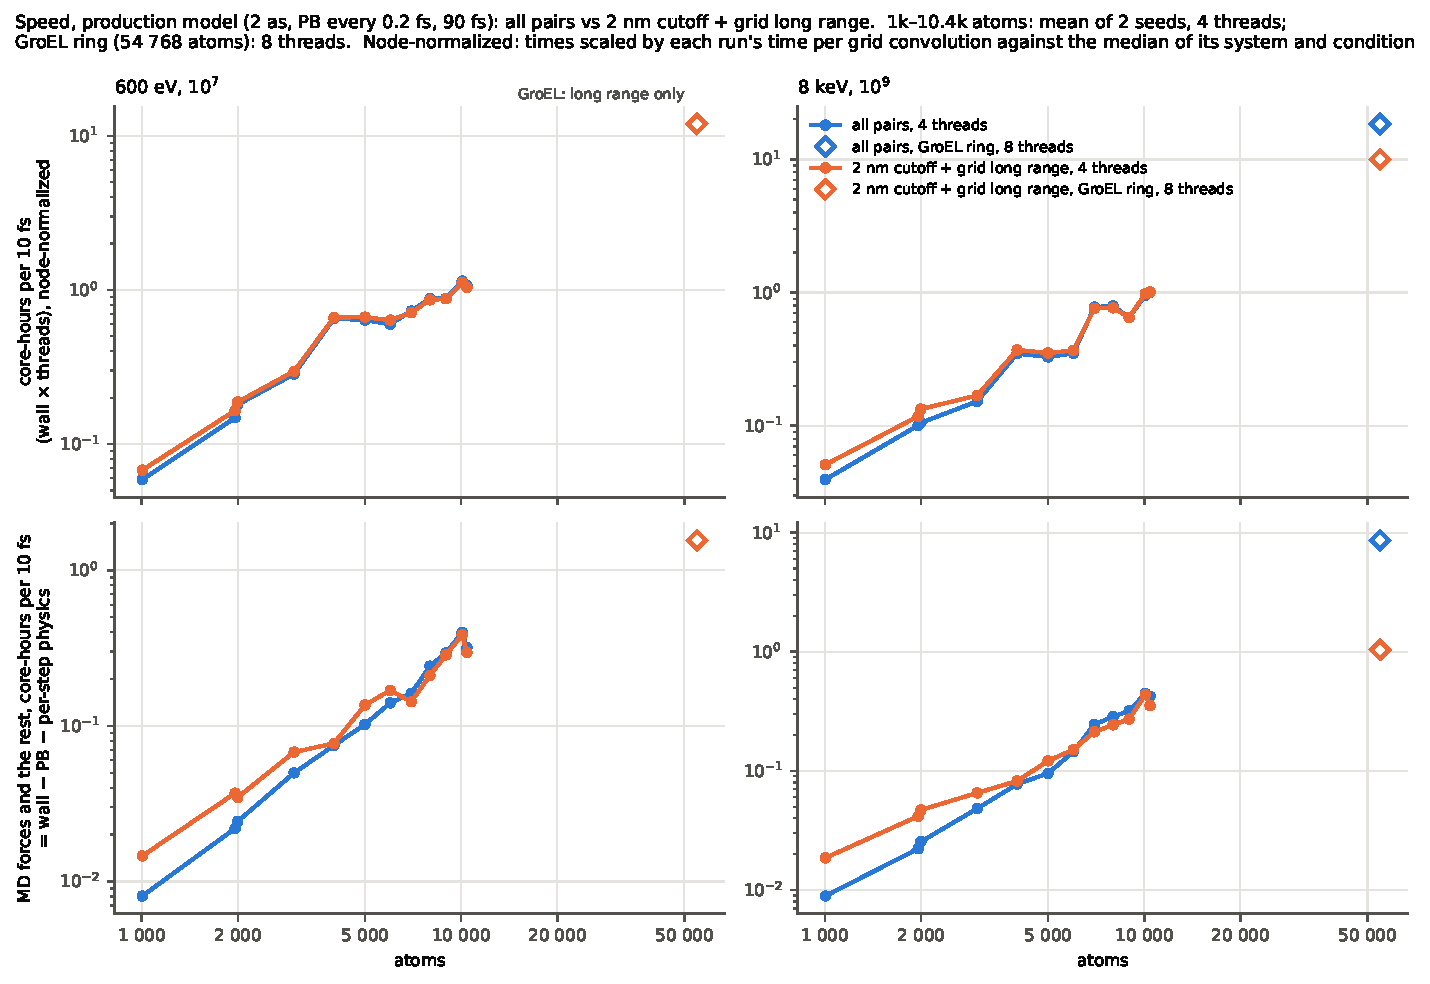
\includegraphics[width=\textwidth]{fig/size_benchmark_speed.pdf}
  \caption{Cost of the production model against system size (core-hours per 10\,fs, node-normalized): all pairs
  against the 2\,nm cutoff plus grid long range. 1k--10k atoms: 4 threads, mean of 2 seeds; GroEL: 8 threads.
  Bottom: the MD forces and the rest, without the PB solve.}
  \label{fig:speed}
\end{figure}
